

\section{Componentes Eletrônicos 2}
\label{componentes_2}


\begin{table}[ht!]

	\begin{tabular}{r l|l p{12cm} }
		
		\textcolor{gray}{Especificação} &&& 	{Componentes Eletrônicos 2}\\
		\textcolor{gray}{Data} &&& 				{14/07/2014}\\
        \textcolor{gray}{Beneficiado} &&&		{Farnell Newark Brasil Distr. de
        Prod. Eletr. LTDA}
        \\
        \textcolor{gray}{CNPJ} &&& 				{01.949.458/0001-54} \\
        \textcolor{gray}{Número Nota} &&& 		{321035} \\
		\textcolor{gray}{Quantidade} &&& 		{-} \\
		\textcolor{gray}{Valor} &&& 			{R\$761,17} \\
		\textcolor{gray}{Data Sheet} &&& 		{-} \\

		\textcolor{gray}{Função no projeto} &&& {Os componentes eletrônicos 2 são
		compostos por : resistores, capacitores cerâmicos, chips conversores de
		comunicação RS232, RS485, conversor ADC, regulador de voltagem,
		microcontroladores, transistores e cristal oscilador. Os componentes serão
		utilizados para a montagem parcial da placa de testes e da placa final da
		eletrônica embarcada. O detalhamento individual da função de cada componente
		eletrônico é realizado no relatório da placa eletrônica customizada.}
		\\
		\textcolor{gray}{Razão da Escolha} &&& {-}

	\end{tabular}
\end{table}

\newpage


\subsection{Nota Fiscal}
\begin{figure}[H]
 \centering
 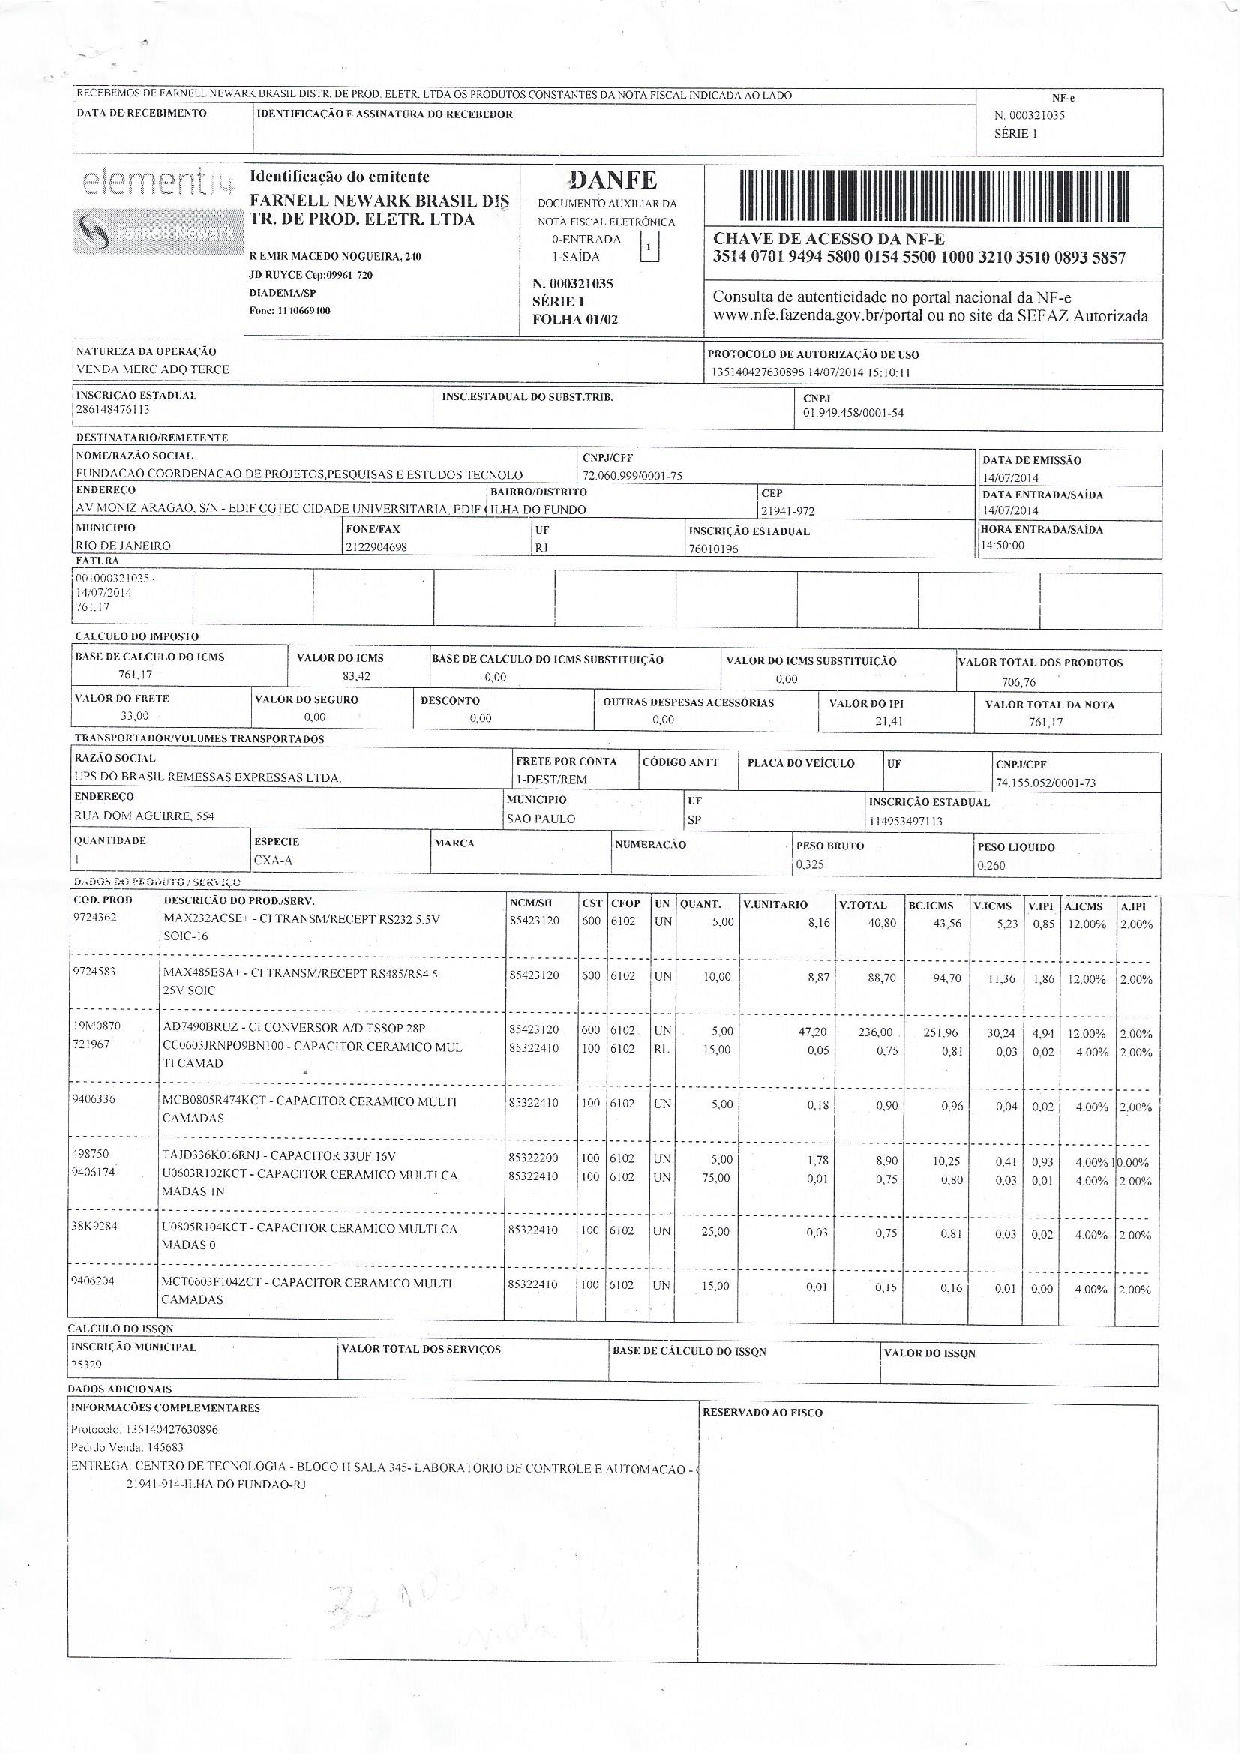
\includegraphics[width=1\columnwidth]{Componentes_Eletronicos_2/nota_eletronica2.pdf}
 \caption{Componentes Eletrônicos 2}
 \end{figure}